%% This is file `sample-sigconf-authordraft.tex',
%% generated with the docstrip utility.
%%
%% The original source files were:
%%
%% samples.dtx  (with options: `all,proceedings,bibtex,authordraft')
%% 
%% IMPORTANT NOTICE:
%% 
%% For the copyright see the source file.
%% 
%% Any modified versions of this file must be renamed
%% with new filenames distinct from sample-sigconf-authordraft.tex.
%% 
%% For distribution of the original source see the terms
%% for copying and modification in the file samples.dtx.
%% 
%% This generated file may be distributed as long as the
%% original source files, as listed above, are part of the
%% same distribution. (The sources need not necessarily be
%% in the same archive or directory.)
%%
%%
%% Commands for TeXCount
%TC:macro \cite [option:text,text]
%TC:macro \citep [option:text,text]
%TC:macro \citet [option:text,text]
%TC:envir table 0 1
%TC:envir table* 0 1
%TC:envir tabular [ignore] word
%TC:envir displaymath 0 word
%TC:envir math 0 word
%TC:envir comment 0 0
%%
%% The first command in your LaTeX source must be the \documentclass
%% command.
%%
%% For submission and review of your manuscript please change the
%% command to \documentclass[manuscript, screen, review]{acmart}.
%%
%% When submitting camera ready or to TAPS, please change the command
%% to \documentclass[sigconf]{acmart} or whichever template is required
%% for your publication.
%%
%%
\documentclass[sigconf]{acmart}
\usepackage{float}
\usepackage{placeins}
\title{Post CMOS technologies: An Overview and Analysis}
%%
%% \BibTeX command to typeset BibTeX logo in the docs
\AtBeginDocument{%
  \providecommand\BibTeX{{%
    Bib\TeX}}}

%% Rights management information.  This information is sent to you
%% when you complete the rights form.  These commands have SAMPLE
%% values in them; it is your responsibility as an author to replace
%% the commands and values with those provided to you when you
%% complete the rights form.
\setcopyright{acmlicensed}
\copyrightyear{2025}
\acmYear{2025}
%% These commands are for a PROCEEDINGS abstract or paper.
%%
%%  Uncomment \acmBooktitle if the title of the proceedings is different
%%  from ``Proceedings of ...''!
%%
%%\acmBooktitle{Woodstock '18: ACM Symposium on Neural Gaze Detection,
%%  June 03--05, 2018, Woodstock, NY}


%%
%% Submission ID.
%% Use this when submitting an article to a sponsored event. You'll
%% receive a unique submission ID from the organizers
%% of the event, and this ID should be used as the parameter to this command.
%%\acmSubmissionID{123-A56-BU3}

%%
%% For managing citations, it is recommended to use bibliography
%% files in BibTeX format.
%%
%% You can then either use BibTeX with the ACM-Reference-Format style,
%% or BibLaTeX with the acmnumeric or acmauthoryear sytles, that include
%% support for advanced citation of software artefact from the
%% biblatex-software package, also separately available on CTAN.
%%
%% Look at the sample-*-biblatex.tex files for templates showcasing
%% the biblatex styles.
%%

%%
%% The majority of ACM publications use numbered citations and
%% references.  The command \citestyle{authoryear} switches to the
%% "author year" style.
%%
%% If you are preparing content for an event
%% sponsored by ACM SIGGRAPH, you must use the "author year" style of
%% citations and references.
%% Uncommenting
%% the next command will enable that style.
%%\citestyle{acmauthoryear}


%%
%% end of the preamble, start of the body of the document source.
\begin{document}

%%
%% The "title" command has an optional parameter,
%% allowing the author to define a "short title" to be used in page headers.
\title{Post CMOS technologies: An Overview and Analysis}

%%
%% The "author" command and its associated commands are used to define
%% the authors and their affiliations.
%% Of note is the shared affiliation of the first two authors, and the
%% "authornote" and "authornotemark" commands
%% used to denote shared contribution to the research.
\author{Willson Luo}
\email{willsonluo@ucla.edu}
\affiliation{
  \institution{University of California Los Angeles}
  \city{Los Angeles}
  \state{California}
  \country{USA}
}

%%
%% By default, the full list of authors will be used in the page
%% headers. Often, this list is too long, and will overlap
%% other information printed in the page headers. This command allows
%% the author to define a more concise list
%% of authors' names for this purpose.
%%
%% The abstract is a short summary of the work to be presented in the
%% article.
\begin{abstract}
  The rapid evolution of computing is pushing the limits of traditional 
  silicon-based electronics, necessitating the exploration of 
  novel materials and architectural paradigms. This paper 
  investigates three transformative technologies poised to 
  redefine future computational systems: Carbon Nanotubes 
  (CNTs), Spintronics, and Memristors. We explore how Carbon 
  Nanotube Field-Effect Transistors (CNFETs) offer enhanced 
  performance and energy efficiency by enabling scaling beyond 
  conventional limits, exemplified by the development of 
  sophisticated CNFET-based microprocessors. Concurrently, 
  Spintronics, particularly through Magnetoelectric Spin-Orbit 
  (MESO) devices, promises ultra-low power logic by leveraging 
  electron spin, introducing innovative concepts like majority 
  logic gates. Furthermore, we examine Memristors, which address 
  the Von Neumann bottleneck by integrating memory and processing, 
  facilitating advanced applications in neuromorphic and analog 
  computing, as demonstrated by their use in artificial neural 
  networks and threshold logic gates. While each technology 
  presents unique challenges in fabrication and integration, 
  their distinct advantages offer compelling pathways toward 
  building faster, smaller, and more energy-efficient computing 
  systems for the next generation.
  CMOS.
\end{abstract}

%%
%% The code below is generated by the tool at http://dl.acm.org/ccs.cfm.
%% Please copy and paste the code instead of the example below.
%%
%%
%% Keywords. The author(s) should pick words that accurately describe
%% the work being presented. Separate the keywords with commas.
\keywords{Post-CMOS Technology, Carbon Nanotubes, CNFETs, Spintronics, MESO Devices, 
Memristors, Crossbar Array, In-Memory Computing, Vector Matrix Multiplication, Majority Gate,
3D Integration, Threshold Logic, Analog Computing}
%% A "teaser" image appears between the author and affiliation
%% information and the body of the document, and typically spans the
%% page.

%%
%% This command processes the author and affiliation and title
%% information and builds the first part of the formatted document.
\maketitle

\section{Introduction}
The pursuit of faster, smaller, and more energy-efficient computing
has been a driving force for technological advancement since the 
creation of the transistor. For decades, CMOS (Complementary
metal-oxide-semiconductor) technology has served as the foundation 
of of the modern computer. However, as we continue to approve our 
transistors and approach fundamental limits, the need for novel 
paradigms becomes increasinly urgent. This paper explores three 
technologies that could shape the future of computing: Carbon Nanotubes
(CNTs), Spintronics, and Memristors. Each offers their own 
advantages that address the limitations of silicon transistors,
varying from faster performance to significantly reduced power 
consumption. 

Carbon Nanotubes, with their exceptional electrical and thermal 
properties, present a compelling alternative to silicon in 
field-effect transistors (FETs). The ability to scale devices 
beyond current limits, coupled with high carrier mobility and 
superior heat dissipation, positions Carbon Nanotube FETs (CNFETs) 
as a potential successor for high-performance, low-power logic. 
Recent advancements, such as the development of the RV16X-NANO 
microprocessor at MIT, demonstrate the practical viability of 
CNFET-based computing, showcasing their compatibility with 
existing design methodologies and their ability to execute 
complex instructions.

Beyond simply replacing silicon, Spintronics offers a 
revolutionary approach to information processing by leveraging 
the intrinsic spin of electrons in addition to their charge. 
Magnetoelectric Spin-Orbit (MESO) devices, a key development in 
spintronics, promise ultra-low power logic operations by directly 
coupling electron spin with its movement and enabling control 
through both electrical and magnetic properties. These devices 
offer superior switching energy, lower operating voltages, and 
enhanced logic density, with the potential to implement universal 
logic through majority gates, fundamentally transforming how logic 
functions are conceived and executed.

Finally, Memristors, often described as the "fourth fundamental 
circuit element," introduce a new dimension to computing by 
combining memory and processing capabilities within a single 
device. This integration directly addresses the Von Neumann 
bottleneck, the traditional separation of memory and logic that 
limits computational speed and efficiency. Memristor-based 
threshold logic gates and crossbar arrays hold immense promise 
for neuromorphic and analog computing, enabling highly efficient 
Vector-Matrix Multiplication (VMM) crucial for artificial neural 
networks. While challenges in manufacturing reliability and 
programmability persist, the ability of memristors to store 
multiple bits and their non-volatile nature offer a path toward 
more compact, power-efficient, and brain-inspired computing 
architectures.

This paper will delve into the principles, advancements, and 
challenges associated with each of these transformative technologies, 
highlighting their individual contributions and their collective 
potential to shape the next generation of computing systems.

\section{Carbon Nanotubes (CNTs) for Advanced Electronics}
As the semiconductor continues its pursuit of miniaturization 
and greater performance, the fundamental limits of silicon-based 
transistors become increasingly apparent. This fundamental limit to 
the scaling of traditional transistors has given rise to many 
alternatives among them being Carbon Nanotubes (CNTs), one 
dimensional nanostructures that possess a unique combination of 
characteristics making them highly attractive for advancing 
electronics.

CNTs are composed of graphene sheets rolled into cylindrical tubes
with their structure determining whether they behave as
semiconductors or metals. his tunable electrical property,
coupled with their nanoscale dimensions, 
high carrier mobility, and exceptional thermal conductivity, 
positions CNTs as a compelling material for high-performance 
computing. Their inherent flexibility also opens avenues for 
novel applications beyond traditional rigid electronics. 
This section will delve into the fundamental properties of 
CNTs, explore their application in Carbon Nanotube Field-Effect 
Transistors (CNFETs), highlight recent advancements that 
demonstrate their potential, and discuss the significant 
fabrication challenges that must be overcome for their widespread 
adoption.

\subsection{Fundamental Properties of Carbon Nanotubes}
Carbon nanotubes are made of an allotrope of carbon known as 
graphene.

Their structure can be characterized into to major types.
Single-walled and multi-walled carbon nanotubes. Single-walled 
carbon nanotubes consist of a single graphene sheet rolled into 
a cylinder typically with a diameter between 0.5 to 2.0 
nanometers. Multi-walled carbon nanotubes are comprised of 
multiple concentric graphene cylinders nested within each other. 
Their diameter can extend up to tens of nanometers. 

The electrical properties can also vary depending on the structure 
and chirality (the angle at which the graphene sheet
is rolled up) of the CNTs. This means that a CNT can behave either 
as metals with a high conductivity or semiconductors making them 
suitable for making transistors. 

CNTs also have extremely high thermal conductivity making them
suitable to overcome many of the power limitations of current 
CMOS scaling.

Finally, CNTs are among the strongest and stiffest materials 
known, possessing exceptional tensile strength and elastic 
modulus. Moreover, they are remarkably flexible, capable of 
withstanding considerable mechanical strain without fracturing. 
This flexibility is particularly advantageous for emerging 
flexible electronics and 3D integration \cite{appenzeller2008carbon}. 

\subsection{Carbon Nanotube Field Effect Transistors (CNFETs)}
The ability of semiconductor CNTs to conduct extremely effectively 
and their nanoscale dimensions make them ideal candidates for 
making the channel in field effect transistors. These properties 
allow CNFETs to offer several significant advantages over silicon 
based FETs:
\begin{itemize}
  \item Aggressive Scaling: Their nanoscale dimensions allow for
  device scaling below the 5 nanometer limit.
  \item High Carrier Mobility: The ballistic or near-ballistic 
  transport of carriers within CNTs leads to very high carrier
  mobility, which translates directly to faster switching speeds 
  and improved device performance.
  \item Lower Power Consumption: CNFETs can operate effectively 
  at lower voltages due to their superior electrical 
  characteristics, resulting in significantly reduced power 
  dissipation.
  \item Enhanced Gate Control: As one-dimensional materials, 
  CNTs offer excellent electrostatic control by the gate, 
  leading to lower off-state currents and steeper subthreshold 
  swings.
  \item Superior Thermal Management: Their high thermal 
  conductivity facilitates efficient heat dissipation, 
  mitigating hot spots and improving reliability in densely 
  packed circuits.
  \item Material Flexibility: The mechanical flexibility of CNTs 
  enables the development of bendable electronics and facilitates 
  potential three-dimensional chip stacking and integration, 
  offering new avenues for compact and innovative designs \cite{javey2003ballistic}.
\end{itemize}

\begin{figure}[h]
  \centering
  \includegraphics[width = \linewidth]{images/Screenshot 2025-05-26 at 8.51.02 PM.png}
  \caption{Diagram of CNFET as combination of MOSFET and FinFET (Image from \cite{appenzeller2008carbon})}
\end{figure}

\subsection{Logic Operations}
Since CNFETs operate just like normal transistors their integration 
into creating logic gates is the exact same as a traditional 
transistor. They still follow CMOS architecture and their benefits 
come from their performance advantage compared to traditional transistors rather than 
new operating paradigms. 

\subsection{Recent Advancements: RV16X-NANO Microprocessor}
The RV16X-NANO Microprocessor has been one of the biggest advancements 
in making a computer with CNFETs. The MIT Medical Electronic Device 
Realization Center were able to develop a 16 bit nanoprocessor which
they named RV16X-NANO. The microprocessor was built of the RISC-V
instruction set which was written through Bluespec and then compiled 
into Verilog, an RTL hardware description langauge. The microprocessor 
was comprised of over 14000 CMOS CNFETs that were made using more than 
10 million CNTs. 

On this microprocessor they were able to implement many standard logic 
blocks like multiplexers, arithmetic logic units, decoders, and encoders. 
Most notably, they were able to execute the famous "Hello World"
program.
\cite{hills2019modern}

\begin{figure}
  \centering
  \includegraphics[width = \linewidth]{images/Screenshot 2025-05-26 at 8.56.27 PM.png}
  \caption{Architecture and Design of RV16X-NANO (Image from \cite{hills2019modern})}
\end{figure}

\subsection{Challenges in CNFET Fabrication and Integration}
Despite the considerable amount of progress made, several challenges 
still need to be addressed before CNFETs can achieve widespread 
viability and meet yield requirements for very large scale integration
(VLSI). Most signficantly, material and manufacturing defects are 
the current biggest challenge. Current methods of CNT fabrication 
lack a reliable way of controlling the chirality leading to many
CNTs exhibiting metallic properties instead of being semiconductors. 
Even after achieving semiconducting CNTs, manufacturing processes still
introduce defects and variability across a wafer. This includes variation
in CNFET density and contact resistance leading to non uniform performance
across an entire chip. In addition to manufacturing issues there 
still lacks a way of seamlessly integrating with traditional silicon
CMOS components\cite{hills2019modern}.
Overcoming these challenges is crucial to achieving reliable CNFETs
capable of making more advanced computers. 


\subsection{Personal Thoughts}
Overall CNFETs seem like a very promising area where there could be 
a lot of development. Since it doesn't deviate signficantly from 
traditional transistors it can be implemented into already made 
computing schemes making it more appealing for companies to invest 
in. It is much more likely for top fabrication companies like 
TSMC or Intel to look into CNFETs than some other technologies
that present completely new computing paradigms. The progress made in 
CNFETs has also been extremely promising as demonstrated by MIT's 
RV16X-NANO computer. The milestone to already have demonstrated 
such funcionality proves that this is a technology that is really 
feasible for the future. Graphene is also an area that has a good 
amount of research going into it so carbon nanotubes in general 
are sure to get more attention. 

With new chips there is a greater emphasis on chiplet technology 
as well as 3D integration. Again, CNFETs look very promising in that
area. Along with that, the medical industry is also constantly looking 
for flexible devices that can better interact with the human body 
which is another area where CNFETs shine in. 

Though there are still some big hurdles to overcome in manufacturing 
CNFETs at large scales and reliably I believe with just a few more 
breakthroughs they can become quite mainstream where large amounts 
of investments will be poured into CNFETs and accelerate their development 
greatly. 

\section{Spintronics: Beyond Charge-Based Computing}
Traditional electronics primarily rely on the charge of electrons 
to process and store information. 1s and 0s are coded by high and 
low volages which are determined by electric fields created by
distributions of charges. However, this approach faces inherent 
limitations in terms of power consumption and switching speed as 
devices continue to shrink. Spintronics emerges as a new paradigm 
that seeks to overcome these limitations by exploiting not only electron's 
charge but also its intrinsic angular momentum, known as spin. 
This additional degree of freedom offers the potential for 
fundamentally new device functionalities, leading to 
ultra-low power consumption, higher operating speeds, and increased 
logic density.

\subsection{Introduction to Spintronics}
Spintronics is the study and exploitation of the spin 
of electrons in solid-state devices. Unlike charge, which is a 
scalar quantity, spin is a quantum mechanical property that can 
be oriented in different directions (e.g., "spin-up" or "spin-down").
This allows for the encoding of information in a non-volatile magnetic
state. The promise of spintronics lies in its ability to enable 
novel functionalities and overcome the inherent energy dissipation 
associated with moving charges in conventional electronics. By manipulating 
spin currents and magnetic states, spintronic devices aim to perform logic 
operations with significantly reduced energy footprints. 
By also utilizing using a charge as well as spin this gives the potential to encode more 
states where there can be a combination of high or low voltage along 
with up or down spin. 


\subsection{Magnetoelectric Spin-Orbit (MESO) Devices} 
One promising way to compute and perform logic using spintronics is 
Magnetoelectric Spin-Orbit (MESO). In this scheme binary is represented 
in the up or down spin state of a nanomagnet. These devices rely 
on 2 major physical effects. The first is spin-orbit transduction where 
if a current flows through a material with a strongly coupled spin 
the current will also gain that spin. The second effect is magnetoelectric 
switching where you can control a materials magnetic properties by applying 
an electric field. For instance switching the spin state with the help of 
an electric field.

\begin{figure}[h]
  \centering
  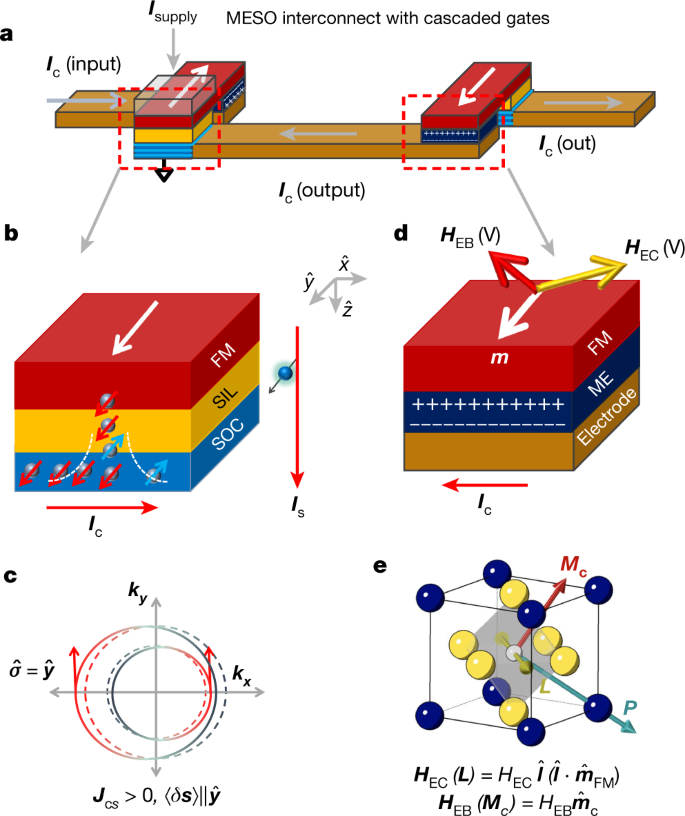
\includegraphics[width = \linewidth]{images/41586_2018_770_Fig2_HTML.png}
  \caption{MESO Spin Device Diagram illustrating various operating mechanisms (image from 
  \cite{manipatruni2019scalable})}
\end{figure}

\subsubsection{Principle of Operation}
The input logic is provided as an electrical charge or voltage. 
This input is applied to a magnetoelectric switching node, which 
can change the magnetization direction of the nanomagnet using a 
voltage. This effectively converts the electrical input into a 
stable magnetic state (representing a 0 or 1 based on its up or 
down spin), which represents the logic state. This form of 
"collective state switching" offers superior switching energy, 
lower operating voltage, and enhanced logic density compared to 
charge-only approaches.

The output logic is then generated by supplying a current into 
the device. The magnetic state of the nanomagnet then determines 
sets all the ejected electrons to be strongly polarized due to spin
orbit coupling. This spin is then converted back into a charge 
or voltage driving the subsequent logic gates. 

\subsubsection{Logic Implementation and Architecture}
The key feature enabling logic implementation with MESO is due to 
their ability to implement majority gates and inverters. MESO devices
inherently suppport majority logic because of the way multiple 
charge inputs can be summed together to influence the spin state
of a nanomagnet. If the spin of the currents sum to be above a 
certain threshold then that will be enough to change the spin state
of the nanomagnet. 

An inverter can then be created by having a nanomagnet affect the 
spin polarization of a wire. If a wire is placed close to a nanomagnet, 
the nanomagnet will act as a sort of a filter. The nanomagnet 
will affect the wire is such a way that electrons with the same spin 
as the magnet will be attracted to the nanomagnet while electrons with 
opposite spin are able to pass through. This then effectively 
outputs a spin state that is opposite to the spin state of 
the nanomagnet creating an inverter. 

These devices can then be cascaded together to perform more advanced 
logic operations. While there still hasn't been much 
substantial demonstration of this technology the theory is there 
and complicated logic operations are definitely possible.
\cite{manipatruni2019scalable}

\subsection{Current Challenges in Spintronics}
Despite the significant theoretical advantages of MESO devices, there 
still stands considerable challengs to it's implementation. The primary 
hurdle still lies in the fact that these devices cannot be produced reliably. 
Temperature fluctuations also pose a significant threat to MESO devices
as shifts in temperature can alter the spin states of the devices. 

\subsection{Personal Thoughts}
While spintronics has a lot of promising benefits with its low power 
and in memory compute, the possibility of an actual computer being 
made with spintronics seems extremeley slim. The current state 
that devices can be manufactured will be nowhere close to the 
reliability needed for spintronics computers. Even in the case that 
an actual computer can be made, it will definitely not be applicable 
to home personal use due to the sensitivity of the devices and how easily 
the spin could change. 

The operating principles behind spintronics inherently seems very
volatile. Much like quantum computing, for it to be viable I think 
extensive error correction algorithms will have to be used that will 
take up a signficant amount of the compute available. The principles 
also make it seem very difficult for the devices to be manufactured at 
a scale comparable to current transistors. I think if spintronics 
logic is to become a thing there may need to be different ways to 
perform logic that is more robust and error tolerant and also perhaps 
a bit more simple. 

There is also not much action if at all happening in industry 
related to spintronics. Companies are still unwilling to invest 
in which is a big indicator in how far off from deployment the 
technology still is. 

Overall, I don't think spintronics will be very viable in performing 
digital logic operations. It may have big potential in spaces like 
memory, but just for logic I don't see it getting very far. If we don't 
see any big advancements in the next 3-5 years I think the research 
and investment around this technology will fall off and people 
will invest all resources to quantum computing. 

\section{Memristors}
The Von Neumann architecture, which physically separates the processing 
unit from the memory has been the preferred method for making computers. 
However, as our chips become faster bottlenecks from I/O also come up 
where information can't be moved to and from the chip fast enough. Memristors, 
first described as the fourth missing circuit element, offer a way 
to link memory and compute in a single device. This combination opens up
potential for more efficient brain inspired computing, particularly 
in the neuromorphic and analog world. 

\subsection{The Memristor Concept}
A memristor, combination of the words memory and resistor, is a device 
that can have a programmble resistance. It was often described as 
the fourth circuit element because it was believed that magnetic fields 
could be used to change the resistance of these devices. However, recent 
devices don't rely on magnetic fields at all and instead use electric fields 
to change the physical and chemical properties of these devices to program 
the resistance. This property, where it can "remember" its resistance allows 
for non volatile memory and reconfigurable logic without having to change 
the physical connections on a chip.

In addition to these new computing regimes they also offer advantages 
in several other areas. They can be manufactured into nanoscale 
dimensions below those of a silicon transistor allowing for greater scaling 
and higher density integration. Their ability to store memory even 
when power is switched enables lower power consumption. Since they can 
also be programmed into continuous resistance values they have the 
ability to store more than just 1 bit per device. Recent experiments
have shown one memristor being able to store 5-7 bits \cite{papandroulidakis2019practical}. Advances 
in memristors have also demonstrated a high level of CMOS compatability 
allowing them to be used in hybrid structures with traditional CMOS 
devices. 

\subsection{Memristor Based Threshold Logic Gate (TLG)}
Beyond their abilities to store memory, memristors are perfectly suited 
for implementing threshold logic gates. 

\subsubsection{Threshold Logic Gate}
A threshold logic gate is a gate that outputs a high signal if 
an input signal surpasses a certain threshold and outputs low 
otherwise. To give an example simply, imagine the input had a range 
of voltages from 0-9 and there is a threshold voltage of 5. Any
input voltage above high will output a binary high signal from the 
gate and any voltage below will output a low signal. A TLG 
is oftentimes also used to analyze a weighted sum from its inputs 
and see if that is above the threshold. 

With these characteristics a TLG can implement any linearly separable
function. This means that for a given function, there exists a 
dividing line (or hyperplane in higher dimensions) that would 
separate all input combinations to one of two distinct output 
groups. 

This also means that a single TLG can implement a boolean function 
that would require multiple logic gates to realize. For example, a 
majority gate would require at least 4 NAND gates to be realized in 
traditional CMOS design while it can be implemented in just one TLG. 

\begin{figure}
  \centering
  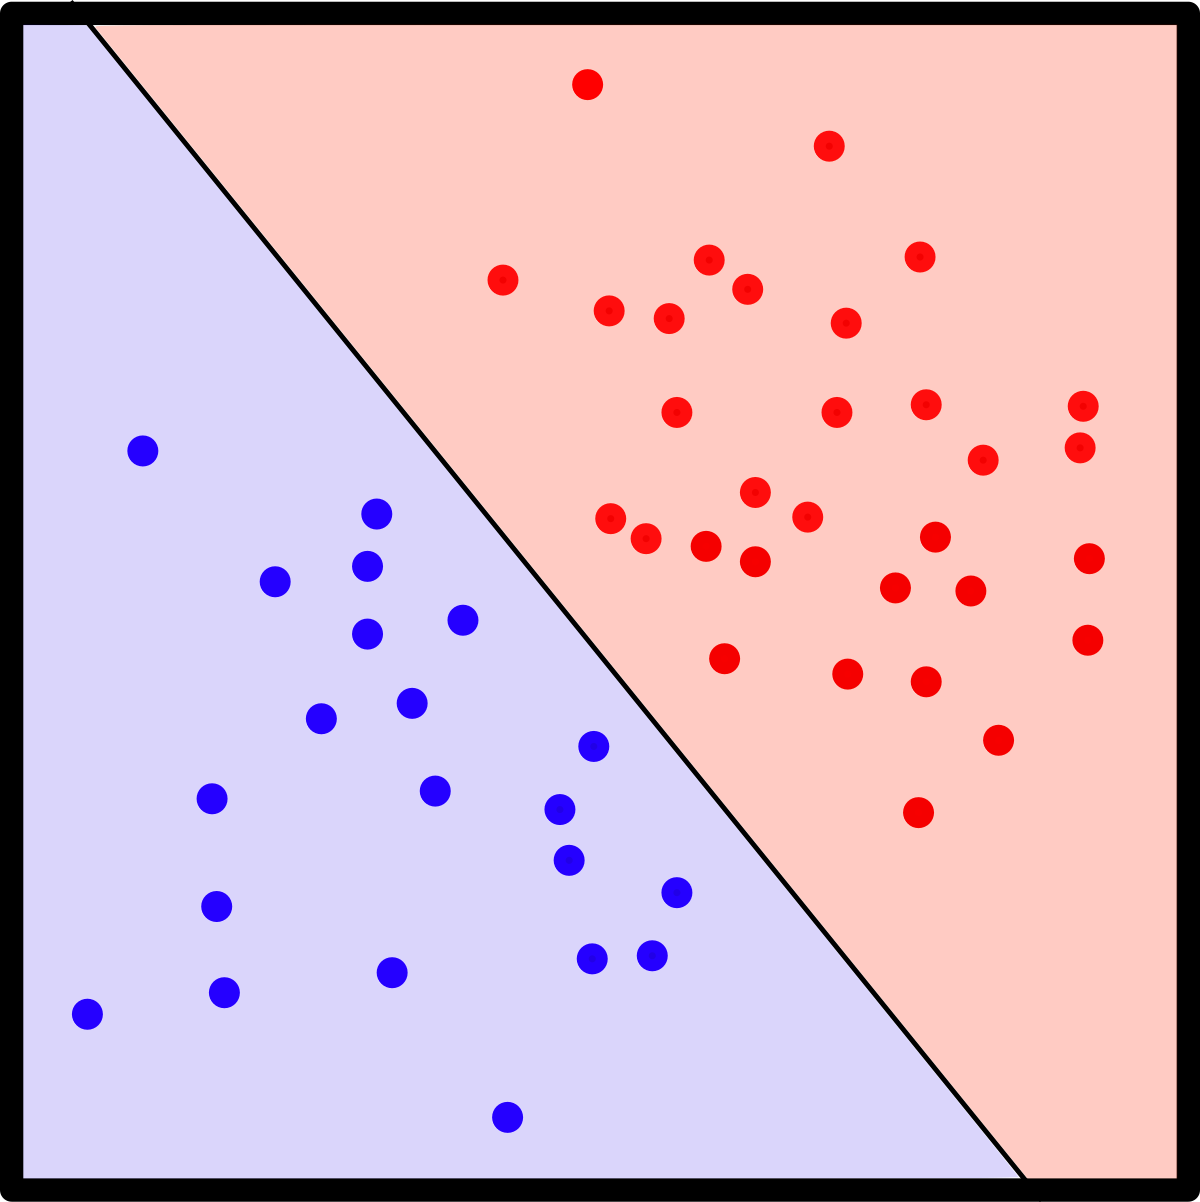
\includegraphics[width = \linewidth]{images/Linearly_separable_red-blue_cropped_.svg.png}
  \caption{Figure illustrating linearly separable function}
\end{figure}

\subsubsection{Memristor-Based Threshold Logic Gate}
Memristors are ideal for TLG implementation since their variable 
resistance can act as programmable weights. A common architecture
for a memristor based TLG implements a hybrid architecture with 
memristors and traditional CMOS components into two main parts:
a differential part and a sensor part. 

The differential part is where a memristor is actually used. Each 
memristor is paired with a transistor known as a 1T1M array.
Here an input and reference threshold signal is taken in. When a 
voltage is then applied as the input current flows through the
memristor. The memristor here acts as a knob that controls how much 
current is passed through this differential part. This part 
can also be switched off when not in use to save power. 

The current from the differential part then goes to the sensor. 
The sensor compares a combined current coming from either one or 
multiple differential parts and sees if its above the threshold. 
Based on this comparison either a 1 or 0 is outputted indicating 
whether the sum of the weights have surpassed the threshold. 
\cite{papandroulidakis2019practical}

\subsubsection{Challenges}
Despite the theoretical efficiency of memristor based TLGs, 
their practical implementation still face significant challenges. 
Fabrication is still very difficult and there are no EDA tools 
compatible with designing devices made of memristors TLGs \cite{papandroulidakis2019practical}. 

\subsection{Hardware Implementation of Memristor-Based Artificial Neural Networks}
Beyond logic gates, memristors are particularly compelling for 
neural networks due to their inherent ability to perform efficient 
vector matrix multiplicaton which serves as the backbone of 
modern neural networks. 

\subsubsection{Vector-Matrix Multiplication (VMM) Core}
The central component in the vector-matrix multiplication core 
is the memristor crossbar array. In this array, memrisotrs are placed
at the crosspoints of a grid of wires. Voltages are inputted through
the rows of the wire and the at each cross point the current is 
found through Ohm's Law. Kirchoff's current law then sums up all the 
currents through the vertical beams and the sum of these currents 
is the result of the vector multiplication. Mathematically the
product as a current is 
\[I_j = \Sigma_iV_iG_{ij}.\]

These raw analog values are then fed to a analog to digital converter
(ADC) to then turn into digital magnitudes. Finally, an activation
function (often a sigmoid or ReLU) is applied to these results to 
introduce nonlinearities, making the output resemble various desired 
distributions \cite{aguirre2024hardware}. 
\begin{figure}[H]
  \centering
  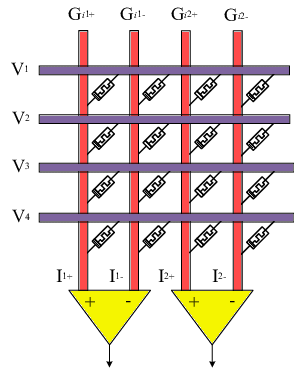
\includegraphics[width = \linewidth]{images/Neural-network-implementation-using-memristor-crossbar-arrays-a-shows-a-conventional.png}
  \caption{Memristor crossbar array (image from \cite{hassan2018real})}
\end{figure}

\subsubsection{Demonstrations of Memristor Neural Networks}
Notably, the University of Michigan created a memristor based 
computer that utilized a 54x108 memristor crossbar array. 
With this computer they were able to create a single layer perception 
that classified a 5x5 array of pixels, identifying the greek letters 
drawn in the 25 pixel array with 100\% accuracy. In addition, they 
implemented a two layer neural network that found commonalities and 
differences in breast cancer screenings, correctly classifying 
the cases as benign or malignant with 94.6\% accuracy.
\cite{cai2019fully}


\begin{figure}[h]
  \centering
  \includegraphics[width = \linewidth]{images/Screenshot 2025-06-07 at 8.22.50 PM.png}
  \caption{Illustration of multiple advances achieved by UMich memristor computer (image from \cite{cai2019fully})}
\end{figure}

\subsection{Challenges to Implementing Memristors}
Despite their demonstrated potential, several critical challenges still
prevent the widespread and practical use of memristors. Among these challenges
the most prominent ones are the lack of reliable manufacturing ability,
resistance drift, and non-linear resistance programming. 

Memristors are still unable to be manufactured reliably and the 
the cost of metal alloys is much more than that of silicon. Manufacturing 
metals to these scales is also much harder. These manufactured devices also 
suffer from drift where the programmed resistance can change over time 
to deviations in the environment like temperature. Non-linearities 
in how the resistance is programmed also make it extremely difficult to
program large scale memristor arrays. Supposed identitical memristors 
could require different voltage thresholds or to be applied for varying 
amount of times to program them to have the same resistance. 

\subsection{Personal Thoughts}
With the advent of AI and the need for massive amounts of compute 
I see memristors having a big potential to fill this opportunity 
to create more powerful and efficient asics for machine learning. 
The development in recent years has also been pretty promising with 
UMich demonstrating the memristor computer implementing a 
single layer perceptron. 

There also seems to be quite a few startups in the space
indicating that memristors may have gotten to the point where 
industry is willing to invest in them. With all the AI startup 
hype these companies are getting massive amounts of money 
and it will boost these companies and the overall memristor fields 
capability to make a breakthrough. 

Outside of making neural networks, I don't think memristors have 
that much viability. The current methods for creating logic gates 
with memristors need quite a lot of traditional CMOS technology to 
support it that it just seems like too much effort for not enough 
benefit. The in memory compute promise also doesn't look too strong
yet and until there can be a way to store significant amounts of memory with 
memristors in the compute block I don't see general purpose memristor 
computers coming anytime soon. 

\section{Comparative Analysis}
This section will then dive into my personal opinions on how these 
technologies compare with each other weighing their respective 
weaknesses and strengths, exploring potential synergies, and consider 
the current landscape of compute and where money and effort is 
being directed. 

The three technologies highlighted above are all among the most 
researched post CMOS technologies in the past few decades. However, 
some definitely have more promise than others. There can 
only be a few winners, and inevitably some will have to fade away 
while others will enjoy widespread adoption. So what exactly are the 
technologies that stand out and in what fields do they have potential. 

First, I will go over which technology I don't think will have 
widespread adoption. That technology would have to be spintronics. 
The main appeal of spintronics is its ability to perform in memory compute. 
This idea is definitely appealing as one of the main bottlenecks that now arise 
scaling compute is the ability to move information to and from memory and compute. 
Spintronics definitely does have its advantanges in this area, however I feel like 
memristors also guarantee this promise in a much more simple and easily conceivable way. 

On the logic side, though spintronics does promise more capable logic abilities with 
the potential of representing more than 2 states in a single bit, the implementation 
just seems too complicated to become scalable. Of course it sounds nice to be able 
to implement more states, but if you're not able to scale this than it's not really 
of any use. Even if scalability is achieved the operating principles behind spintronics 
logic like storing spin states in a nanomagnet are too volatile to be used in anything 
outside of specialized supercomputers. 

On top of all this, the whole field didn't seem to have too many tangible achievements in 
recent times. Research and theory is great, but if none of it can be turned into an actual 
demonstrable product then it really is just theorizing. Unlike the other two technologies 
that have all produced computers that have been able to accomplish some simple and basic tasks
spintronics has not done any of this. 

The technology also doesn't appeal much to the landscape of the industry. With AI being 
all the craze and where all the investment is going, spintroncis doesn't seemed to 
be involved in any of it. 

Carbon nanotubes and memristors on the other hand have much more potential while also 
demonstrating significant results already. Their respective strengths in creating 
hyper-efficient transistors and enabling powerful in-memory computing align directly
with the primary challenges and investment trends in the industry today, making them 
the most compelling candidates to lead the post-CMOS era.

Carbon nanotubes in particular are extremely promising. The benefits they can provide 
are a huge advantage of the transistors we already have. Even though they don't 
present a whole new computing paradigm they still amount to a significant improvement 
in the ability to scale compute. Their ballistic transport properties also make them 
very compelling as it presents ways to reduce power scaling, one of the main factors 
limiting our ability to add more transistors on a chip. 

The results that have already been realized using CNFETs are nothing short of incredible. 
With the MIT Medical Electronic Device Realization center already building a complete 
16 bit computer the promise of carbon nanotubes is no longer just in theory. It is 
knocking on the doorstep ready to take computing to the next step

Because they are not a completely new computing paradigm that also makes it quite appealing. 
With technologies like spintronics and memristors presenting completely new ways to compute
the industry may become hesitant to switch and it will take a significant amount of effort
for everyone to adopt to something so different. Carbon nanotubes on the other hand can operate
just like normal transistors making the transition much more seamless. The difficulty then just 
lies in the fabrication while the rest of the industry can stay more or less the same. 

Perhaps one of the most transformative advantages of carbon nanotubes is their potential 
for true 3D integration. Unlike silicon, which requires high-temperature processing that 
prevents stacking active layers, CNTs can be fabricated at low temperatures. This opens the 
door to building processors vertically, layer by layer, leading to an unprecedented density
of compute and memory interwoven in a single chip. This positions CNTs as the heir apparent 
to silicon for processing tasks.

Finally, memristors who don't have as much potential as carbon nanotubes in the world 
of general have massive potential in the world of specialized AI chips. Their inherent 
ability to do matrix multiplication makes them especially appealing in this day and age 
where training the best AI is what has captivated governments around the world. 

Just like carbon nanotubes, the results that have already been shown using memristors have 
been nothing short of incredible. The University of Michigan implmeneting a single layer 
perceptron also demonstrates that memristors are also not just something of theory. If these 
results can be demonstrated on progressively larger scale models then they have a serious 
chance of taking over the AI industry and becoming the dominant way of making chips in
that space. 

All of this is without even mentioning their potential for in memory compute. Just like 
spintronics, they have the ability to combine memory and compute in the same module and 
if this can be utilized in addition to their matrix multiplication then memristors also 
have a potential chance of brekaing into the general compute space. 

While they are also still quite volatile, just like spintronics, the advancement of 
memristors to become consistent and scalable seem much easier than nanomagnets. Carbon 
nanotubes still stand a step above them in terms of reliability and scalability and are 
ahead in manufacturing maturity. 

In the final analysis, the race to succeed CMOS may not produce a single winner, 
but rather a new, specialized hierarchy of technologies. While spintronics appears to 
be a distant prospect due to fundamental hurdles, the paths for carbon nanotubes and 
memristors are becoming increasingly clear. Carbon nanotubes stand out as the most 
pragmatic and powerful successor for general-purpose logic, promising to extend the 
paradigm of Moore's Law through superior efficiency and 3D integration. They represent 
the perfection of the processor as we know it.

However, perfecting the processor alone is not enough. The future of computing, 
particularly in the age of AI, hinges on solving the data bottleneck. This is where 
memristors, with their profound potential for in-memory and analog computing, will 
dominate. There is a possibility of a hybrid future where efficient logic chips built 
from carbon nanotubes work in seamless integration with memristor based accelerators 
and memory modules. Dividing the labor and letting each technology excel at its 
inherents strengths present a logical and promising path forward. 


\section{Conclusion}
The relentless march of progress in computing has driven 
silicon-based CMOS technology to its fundamental physical limits, 
necessitating a paradigm shift towards novel materials and 
architectural approaches. This paper has explored three 
cutting-edge technologies—Carbon Nanotubes (CNTs), Spintronics, 
and Memristors—each offering distinct and powerful solutions to 
the challenges of performance, power consumption, and 
architectural bottlenecks inherent in current computing systems.

Carbon Nanotubes stand as a compelling successor to silicon in 
transistor technology. Their nanoscale dimensions, exceptional 
carrier mobility, and superior thermal properties enable the 
creation of CNFETs that promise higher speeds, lower power 
consumption, and greater scalability, as evidenced by the 
development of functional CNFET-based microprocessors. While 
significant fabrication hurdles related to material purity and 
manufacturing uniformity remain, the ongoing advancements 
underscore their potential to extend the capabilities of 
traditional digital logic.

Spintronics, by harnessing the intrinsic spin of electrons, 
introduces a revolutionary approach to logic and memory. 
Magnetoelectric Spin-Orbit (MESO) devices demonstrate the 
ability to perform ultra-low-power logic operations by converting 
charge to magnetic states and back, enabling efficient information 
processing with minimal energy dissipation. The inherent 
capability to implement majority gates and inverters fundamentally 
redefines logic design, paving the way for highly dense and 
energy-efficient circuits. Overcoming challenges in gate 
reliability and material integration will be crucial for 
widespread adoption.

Finally, Memristors present a transformative solution to the 
enduring Von Neumann bottleneck by merging memory and processing 
capabilities within a single device. Their unique properties, 
including nanoscale dimensions, non-volatility, and multi-bit 
storage, make them ideal for neuromorphic computing and in-memory 
acceleration of Artificial Neural Networks. The successful 
implementation of memristor-based threshold logic gates and 
complex neural networks showcases their profound potential to 
enable highly efficient, brain-inspired architectures, despite 
ongoing challenges in manufacturing consistency and programming 
precision.

In conclusion, while each of these technologies faces its own set 
of engineering and scientific challenges, their combined potential
is immense. They offer not just incremental improvements but 
pathways to fundamentally reshape how information is processed 
and stored. Whether through the direct performance enhancement of 
CNFETs, the ultra-low-power logic of spintronics, or the 
architectural revolution promised by memristors, the future of 
computing will undoubtedly be a fascinating interplay of these 
emerging paradigms, leading to more intelligent, efficient, and 
powerful computational systems.

%%
%% The acknowledgments section is defined using the "acks" environment
%% (and NOT an unnumbered section). This ensures the proper
%% identification of the section in the article metadata, and the
%% consistent spelling of the heading.
\begin{acks}
This work would not have been possible without the support of Professor Srivastava. None of this paper could 
have come together without your mentorship. Thank you for giving me the opportunity to
research this topic as well. Without this class, I would have never read into this field with such 
depth and it has truly provided me with some valuable insight in addition to skills on 
how to read and analyze papers. 

Of course, this paper would also not have been possible without my classmates. I can say 
confidently that my paper would be nowhere near where it is now had it not 
been for my classmates support and comradery. I have also learned so much through 
each of their presentations. 
\end{acks}

%%
%% The next two lines define the bibliography style to be used, and
%% the bibliography file.
\bibliographystyle{ACM-Reference-Format}
\bibliography{refs}


\end{document}
\endinput
%%
%% End of file `sample-sigconf-authordraft.tex'.